\chapter{Конструкторская часть}

В данном разделе будут представлены схемы алгоритма полного перебора и муравьиного алгоритма.

\section{Требования к ПО}

К программе предъявлены ряд требований:

\begin{itemize}[label=---]
	\item программа должна получать на вход матрицу смежности, для которой можно будет выбрать один из алгоритмов поиска оптимальных путей (полным перебором или муравьиным алгоритмом);
	\item программа должна позволять пользователю определять коэффициенты и количество дней для метода на основе муравьиного алгоритма;
	\item программа должна давать возможность получить минимальную сумму пути, а также сам путь, используя один из алгоритмов.
\end{itemize}

\section{Разработка алгоритмов}

На рисунке~\ref{fig:full-comb} представлена схема алгоритма полного перебора путей.
На рисунках~\ref{fig:ants-1} и \ref{fig:ants-2}  представлена схема муравьиного алгоритма.

\begin{figure}[h]
	\centering
	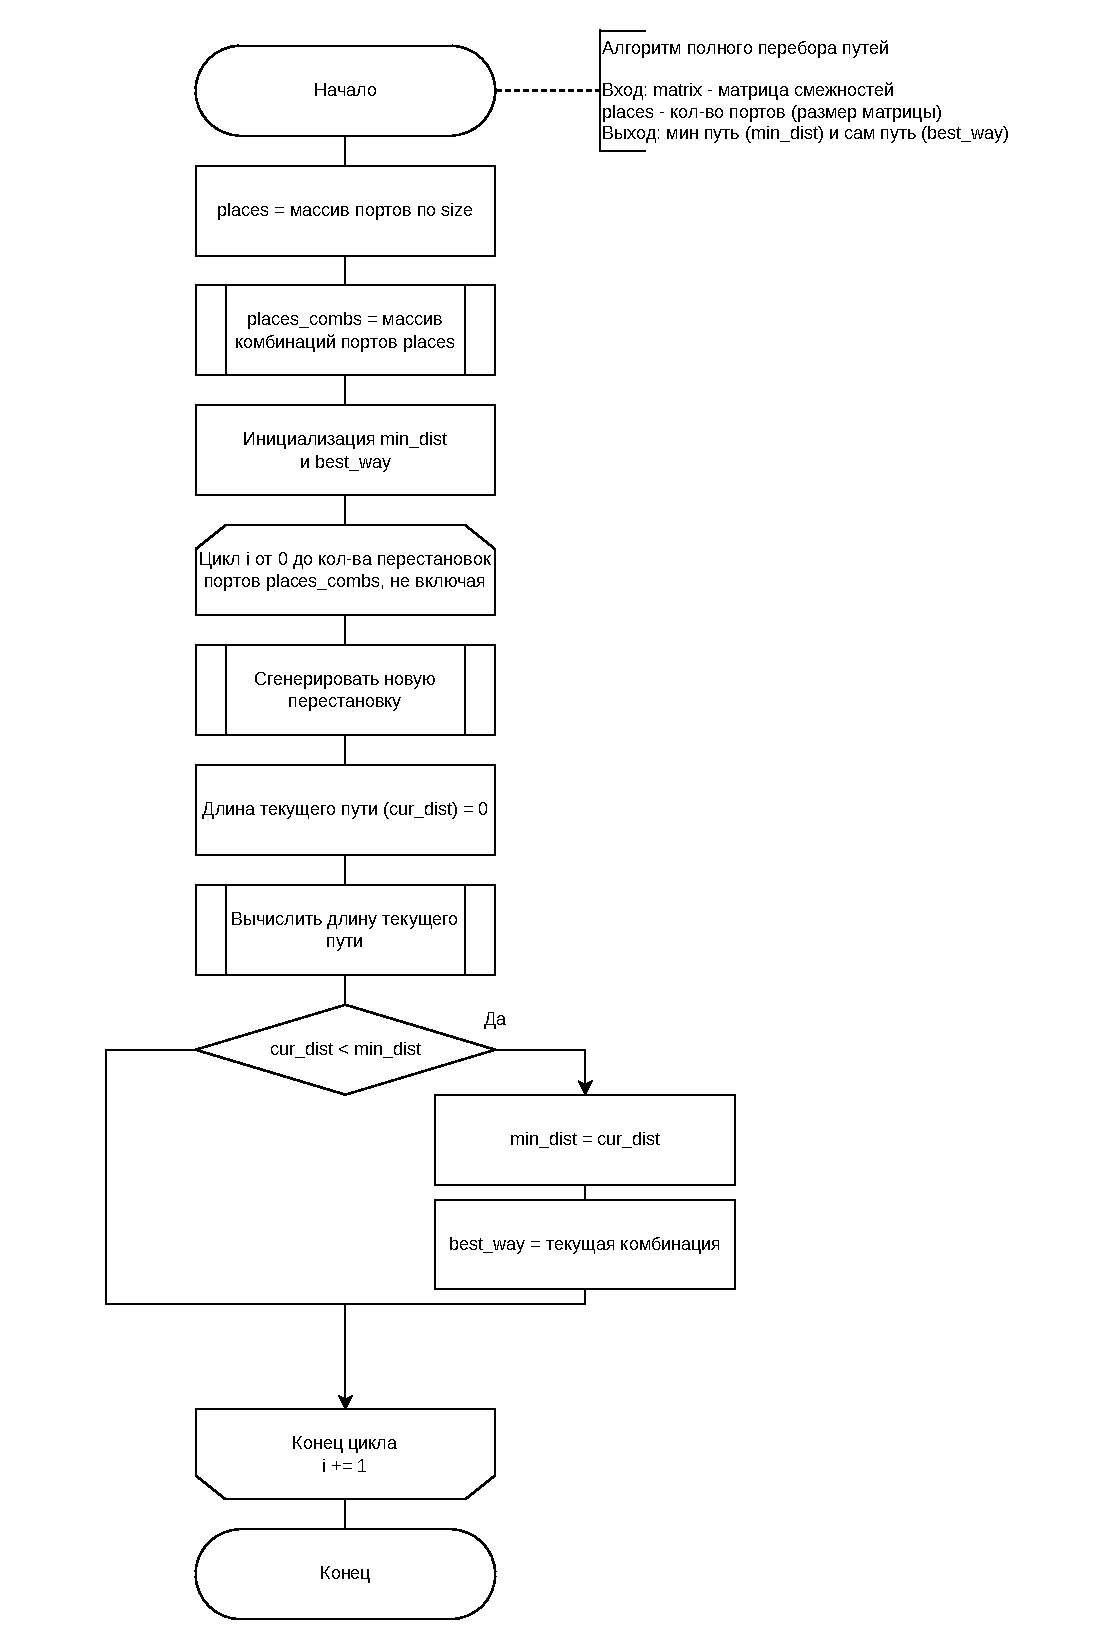
\includegraphics[height=0.8\textheight]{img/full-comb.pdf}
	\caption{Схема алгоритма полного перебора путей}
	\label{fig:full-comb}
\end{figure}

\begin{figure}[h]
	\centering
	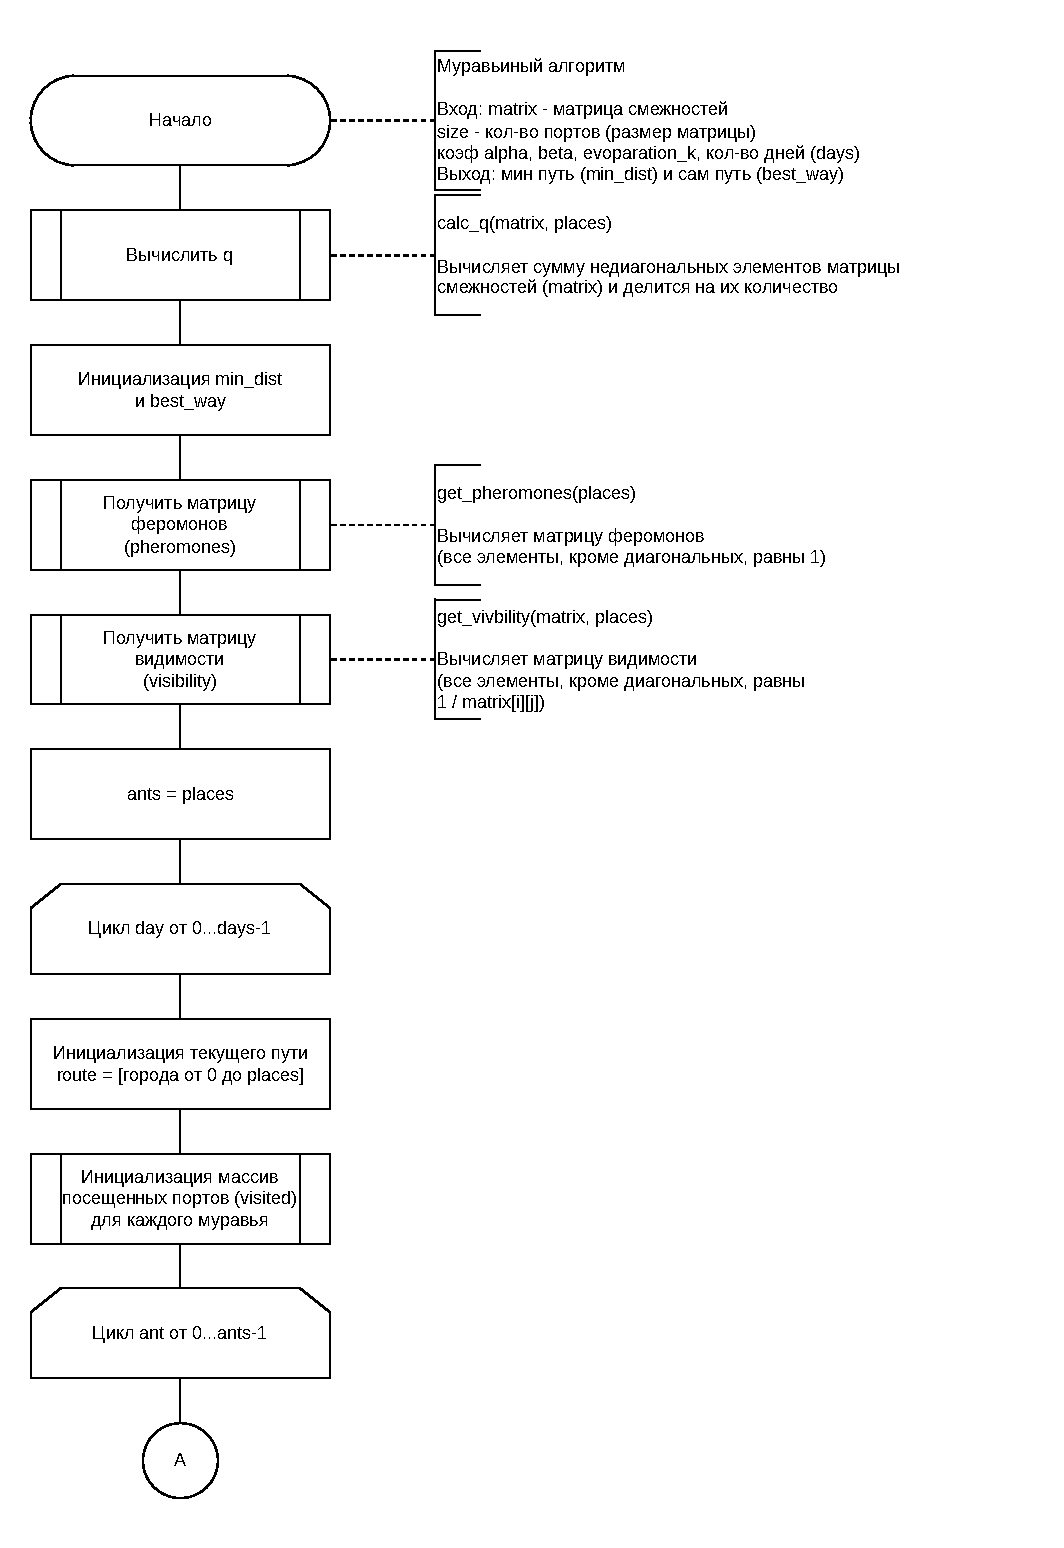
\includegraphics[height=0.9\textheight]{img/ants-1.pdf}
	\caption{Схема муравьиного алгоритма (часть 1)}
	\label{fig:ants-1}
\end{figure}

\begin{figure}[h]
	\centering
	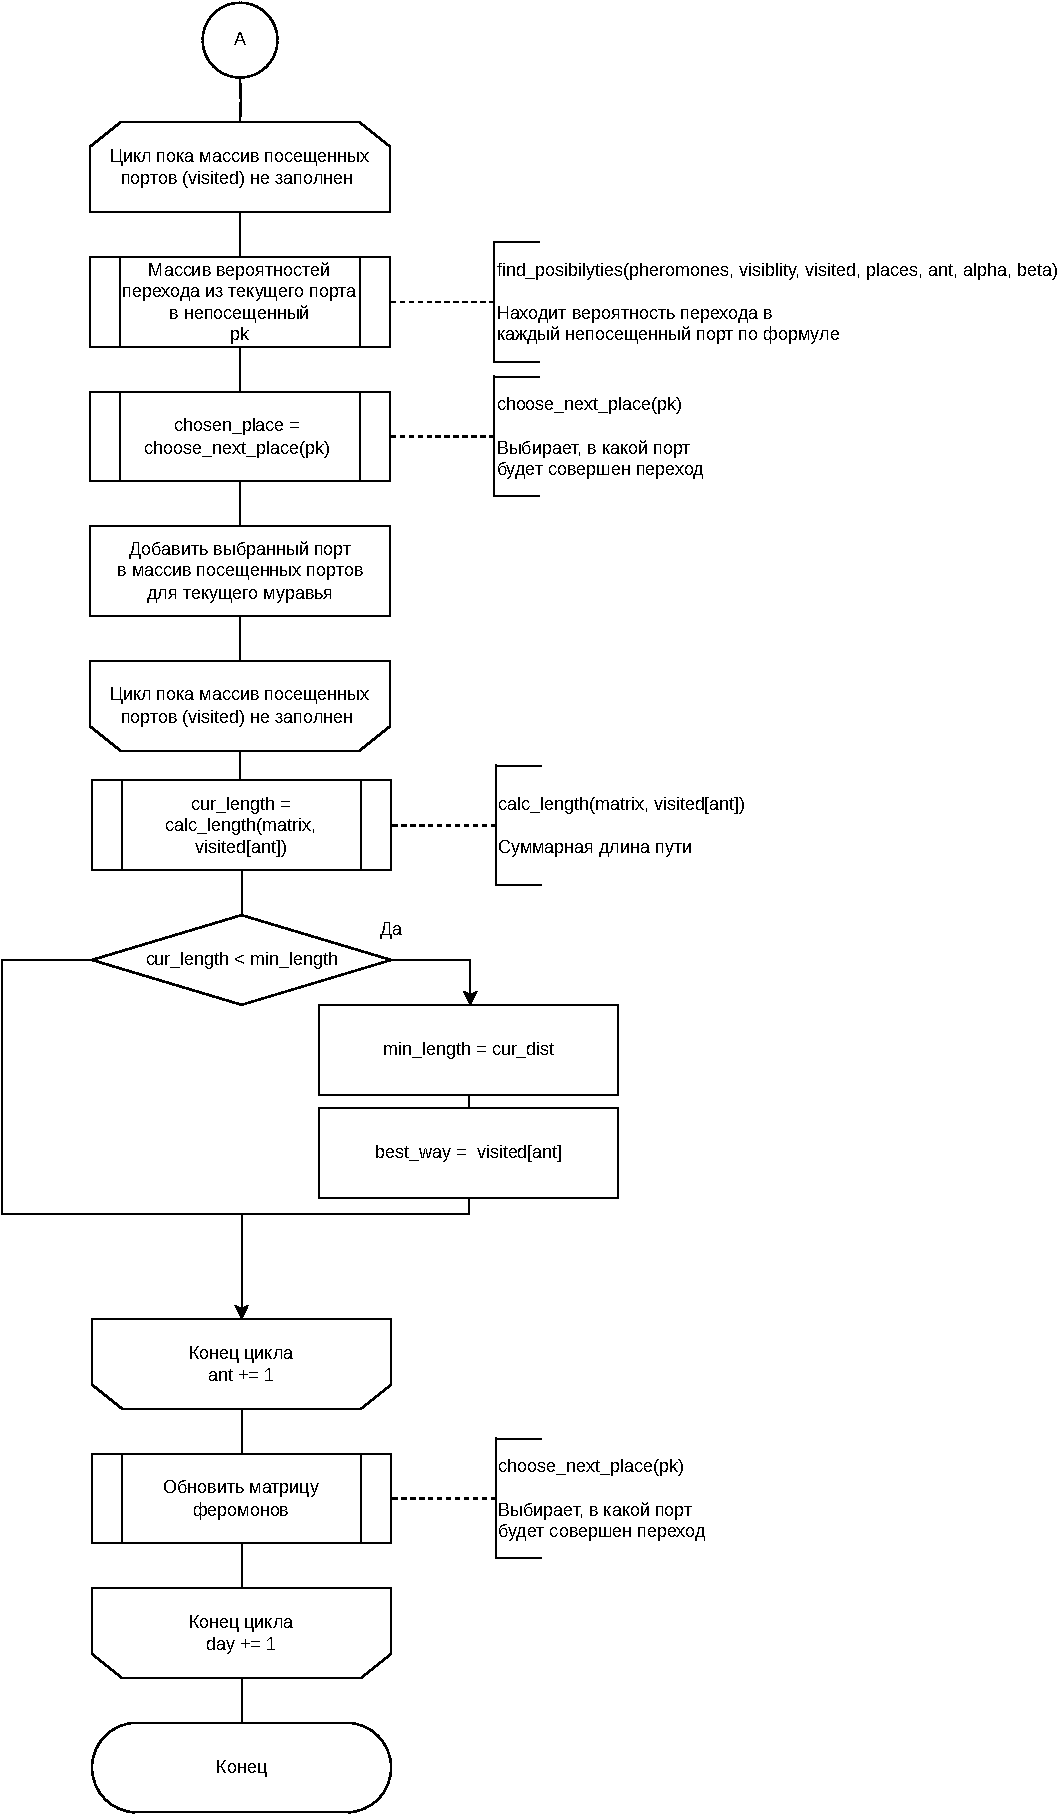
\includegraphics[height=0.9\textheight]{img/ants-2.pdf}
	\caption{Схема муравьиного алгоритма (часть 2)}
	\label{fig:ants-2}
\end{figure}

\begin{figure}[h]
	\centering
	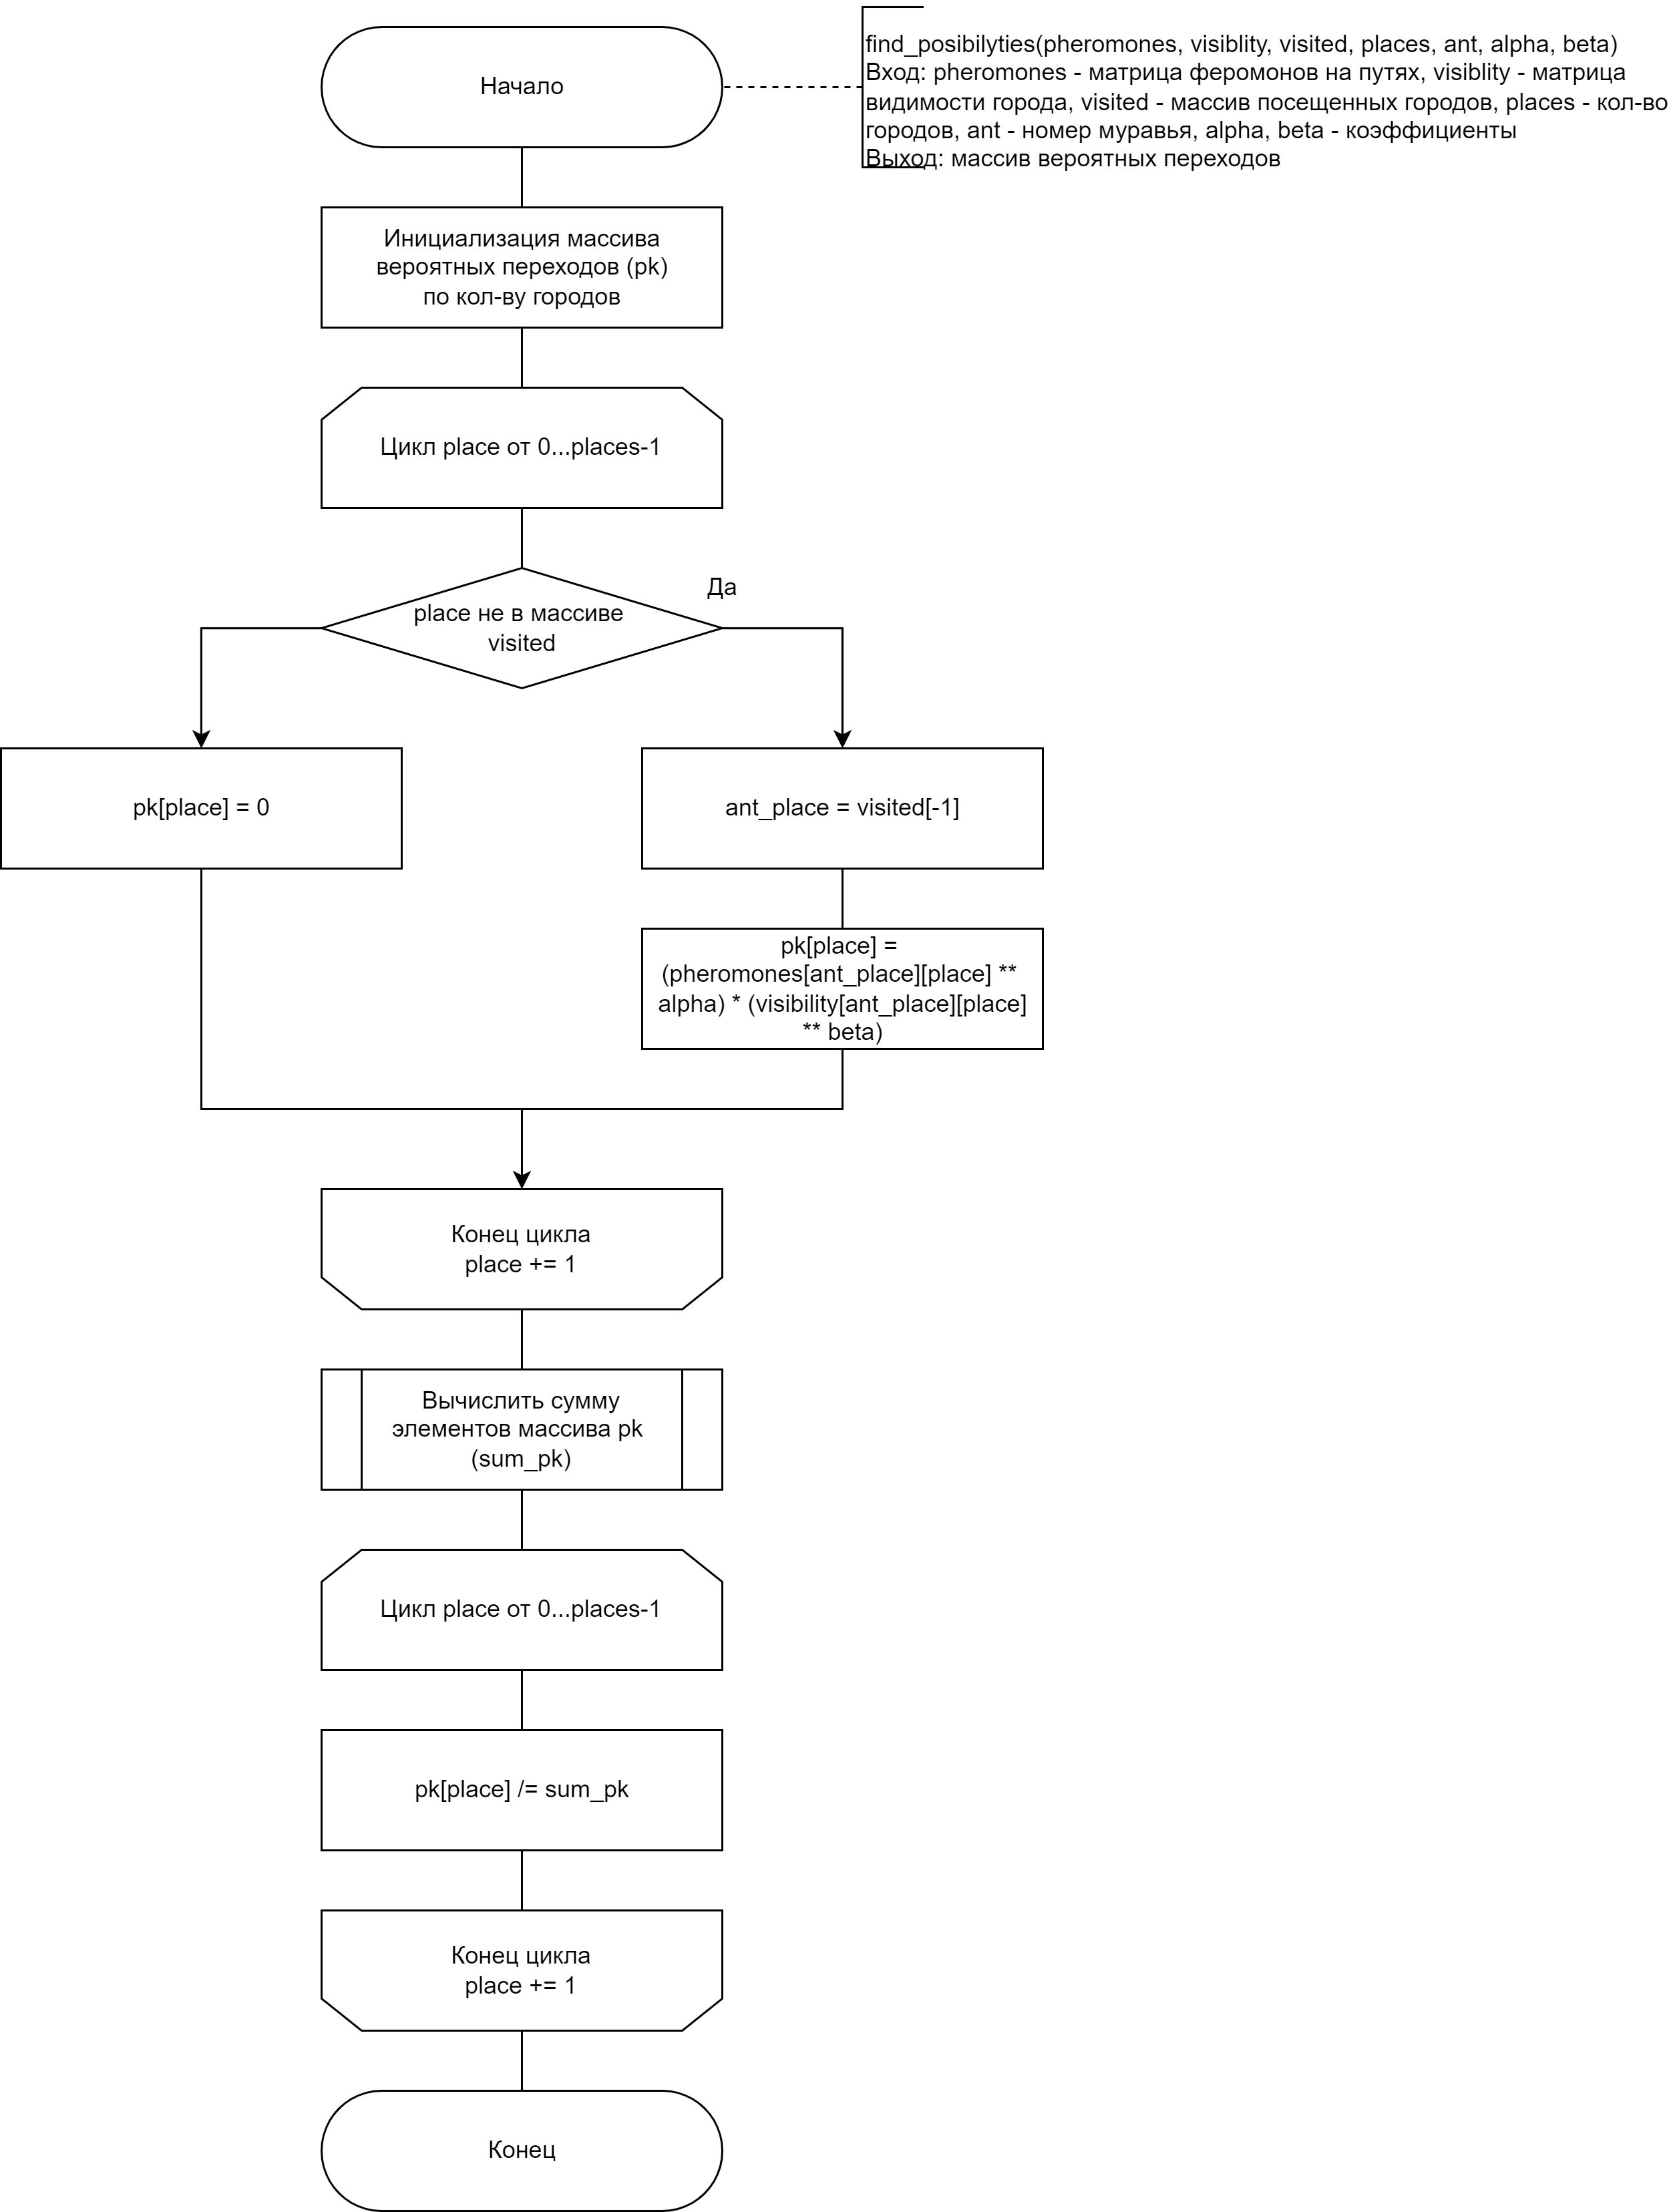
\includegraphics[height=0.9\textheight]{img/find-pos.png}
	\caption{Схема алгоритма нахождения массива вероятностей переходов в непосещенные порты}
	\label{fig:find-pos}
\end{figure}

\begin{figure}[h]
	\centering
	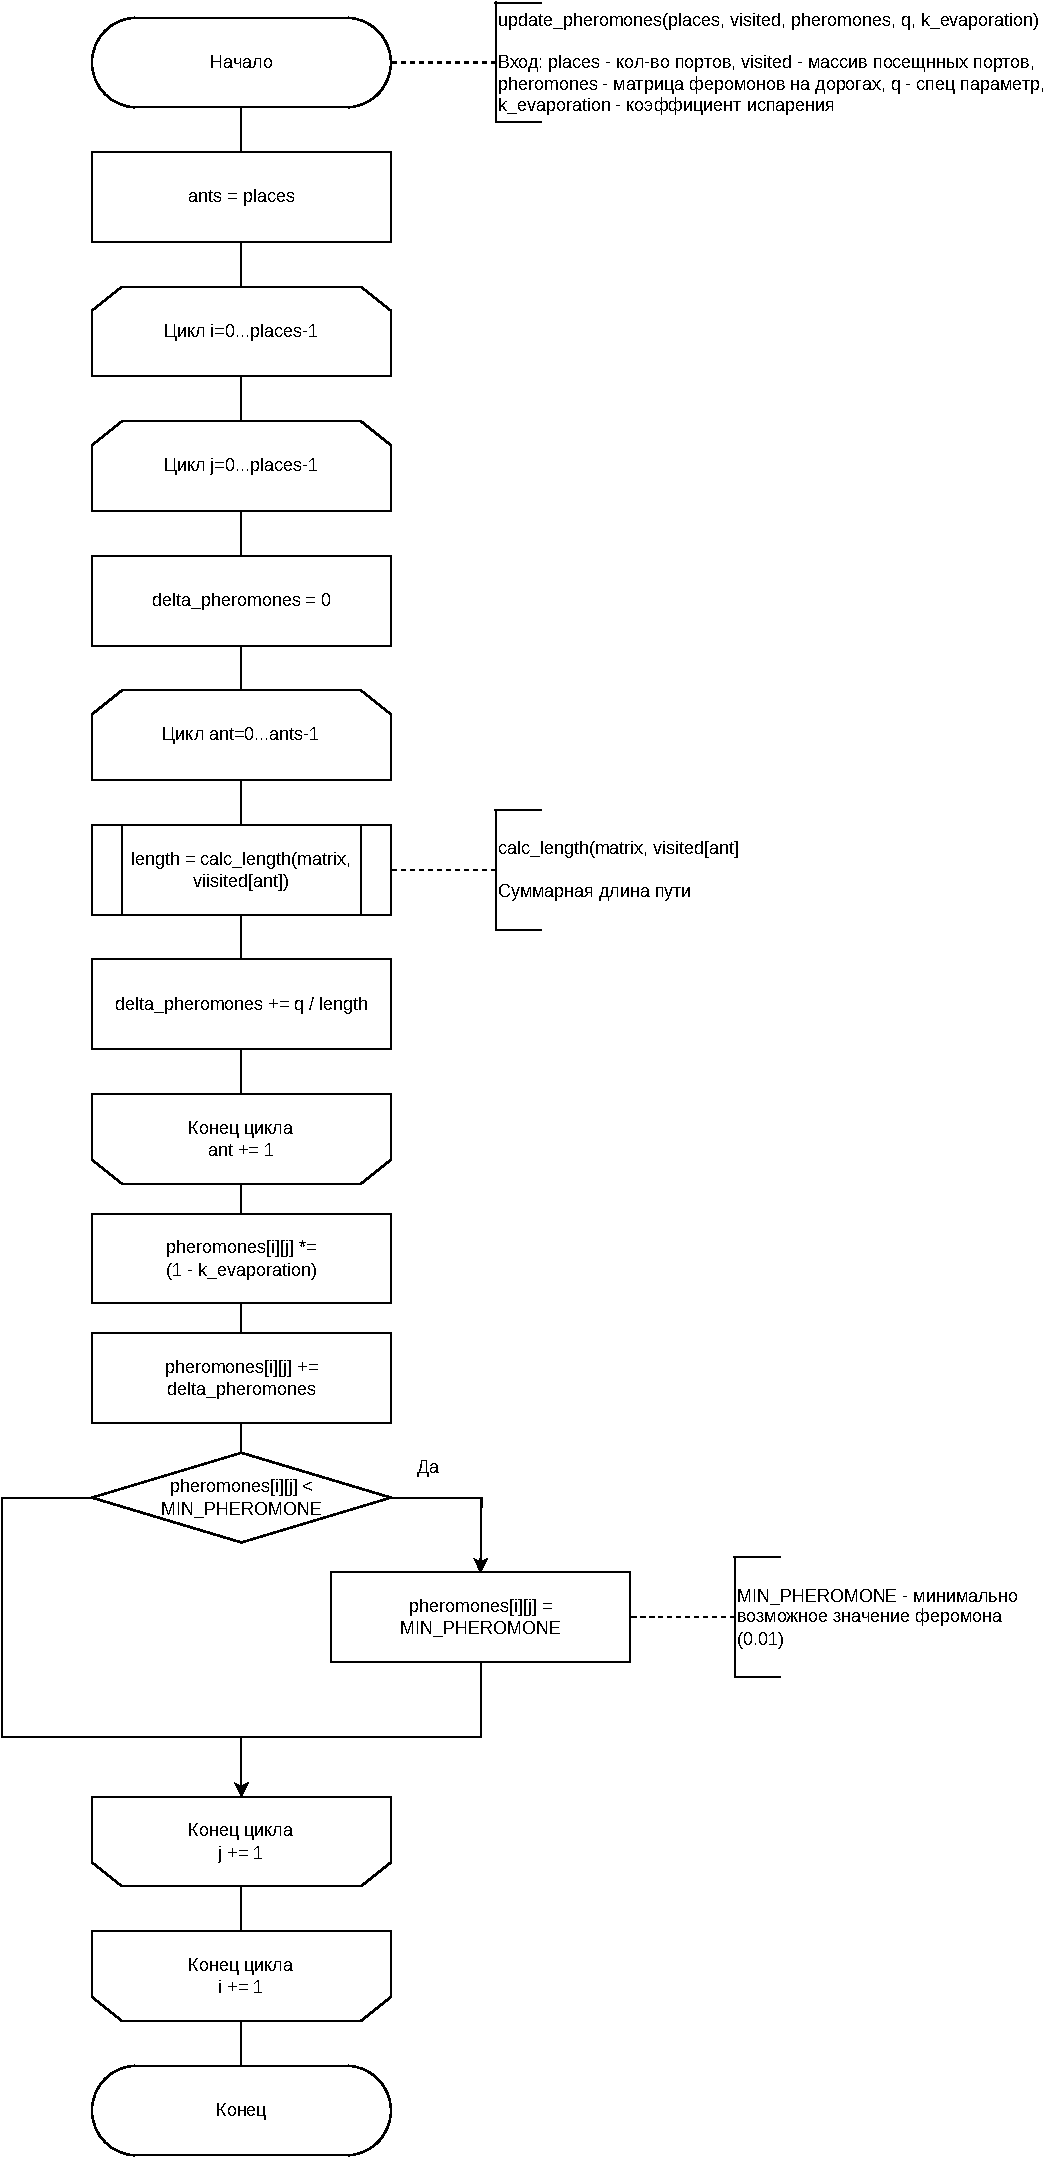
\includegraphics[height=0.9\textheight]{img/update.pdf}
	\caption{Схема алгоритма обновления матрицы феромонов}
	\label{fig:update}
\end{figure}

\begin{figure}[h]
	\centering
	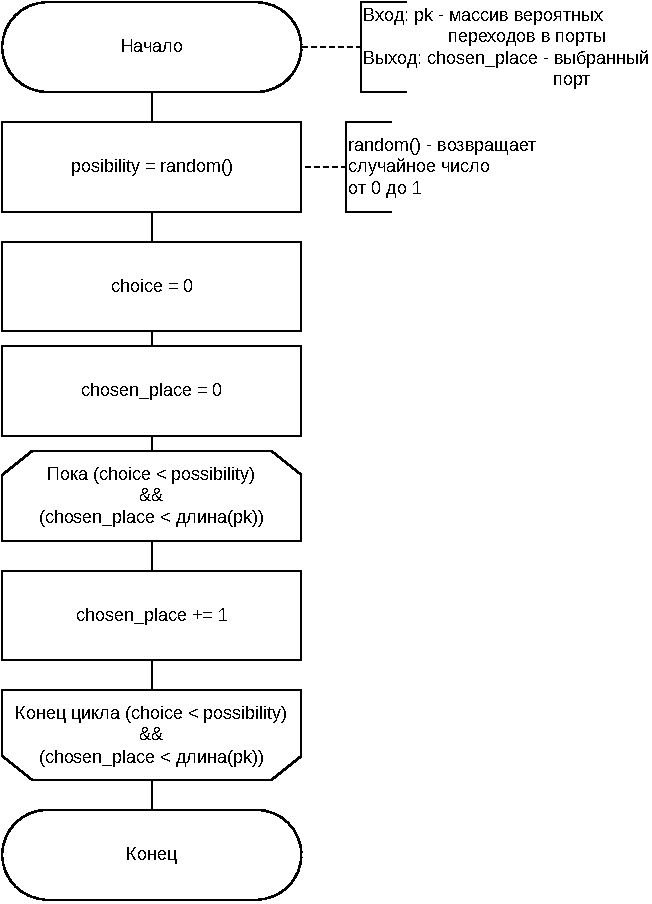
\includegraphics[height=0.7\textheight]{img/rand-choice.pdf}
	\caption{Схема алгоритма выбора следующего порта}
	\label{fig:rand-choice}
\end{figure}

\clearpage

\section{Описание используемых типов данных}
При реализации алгоритмов будут использованы следующие типы данных:
\begin{itemize}[label=---]
	\item размер матрицы смежности --- целое число;
	\item имя файла --- строка;
	\item матрица смежности --- матрица целых чисел.
\end{itemize}

\section*{Вывод}
В данном разделе была рассмотрена задача коммивояжера, а также метод полного перебора для её решения и метода на основе муравьиного алгоритма. Были представлены требования к разрабатываемому программному обеспечению.
